% Para obtener imagénes de tipo vectorial en la plataforma de MATLAB, debes guardar las figuras, como archivo tipo ".eps".

\documentclass{article}
\usepackage{graphicx} % Required for inserting images

\title{IMAGENES VECTORIALES MATLAB}
\author{Giuseppe Fuentes Moreno}
\date{September 2024}

\begin{document}

\maketitle

\section{Introduction}

%Para añadir la imagen vectorial, realizamos el mismo proceso para agregar imagenes con el comandoo "\begin{figure}":
\begin{figure}
\begin{center}
    \centering
    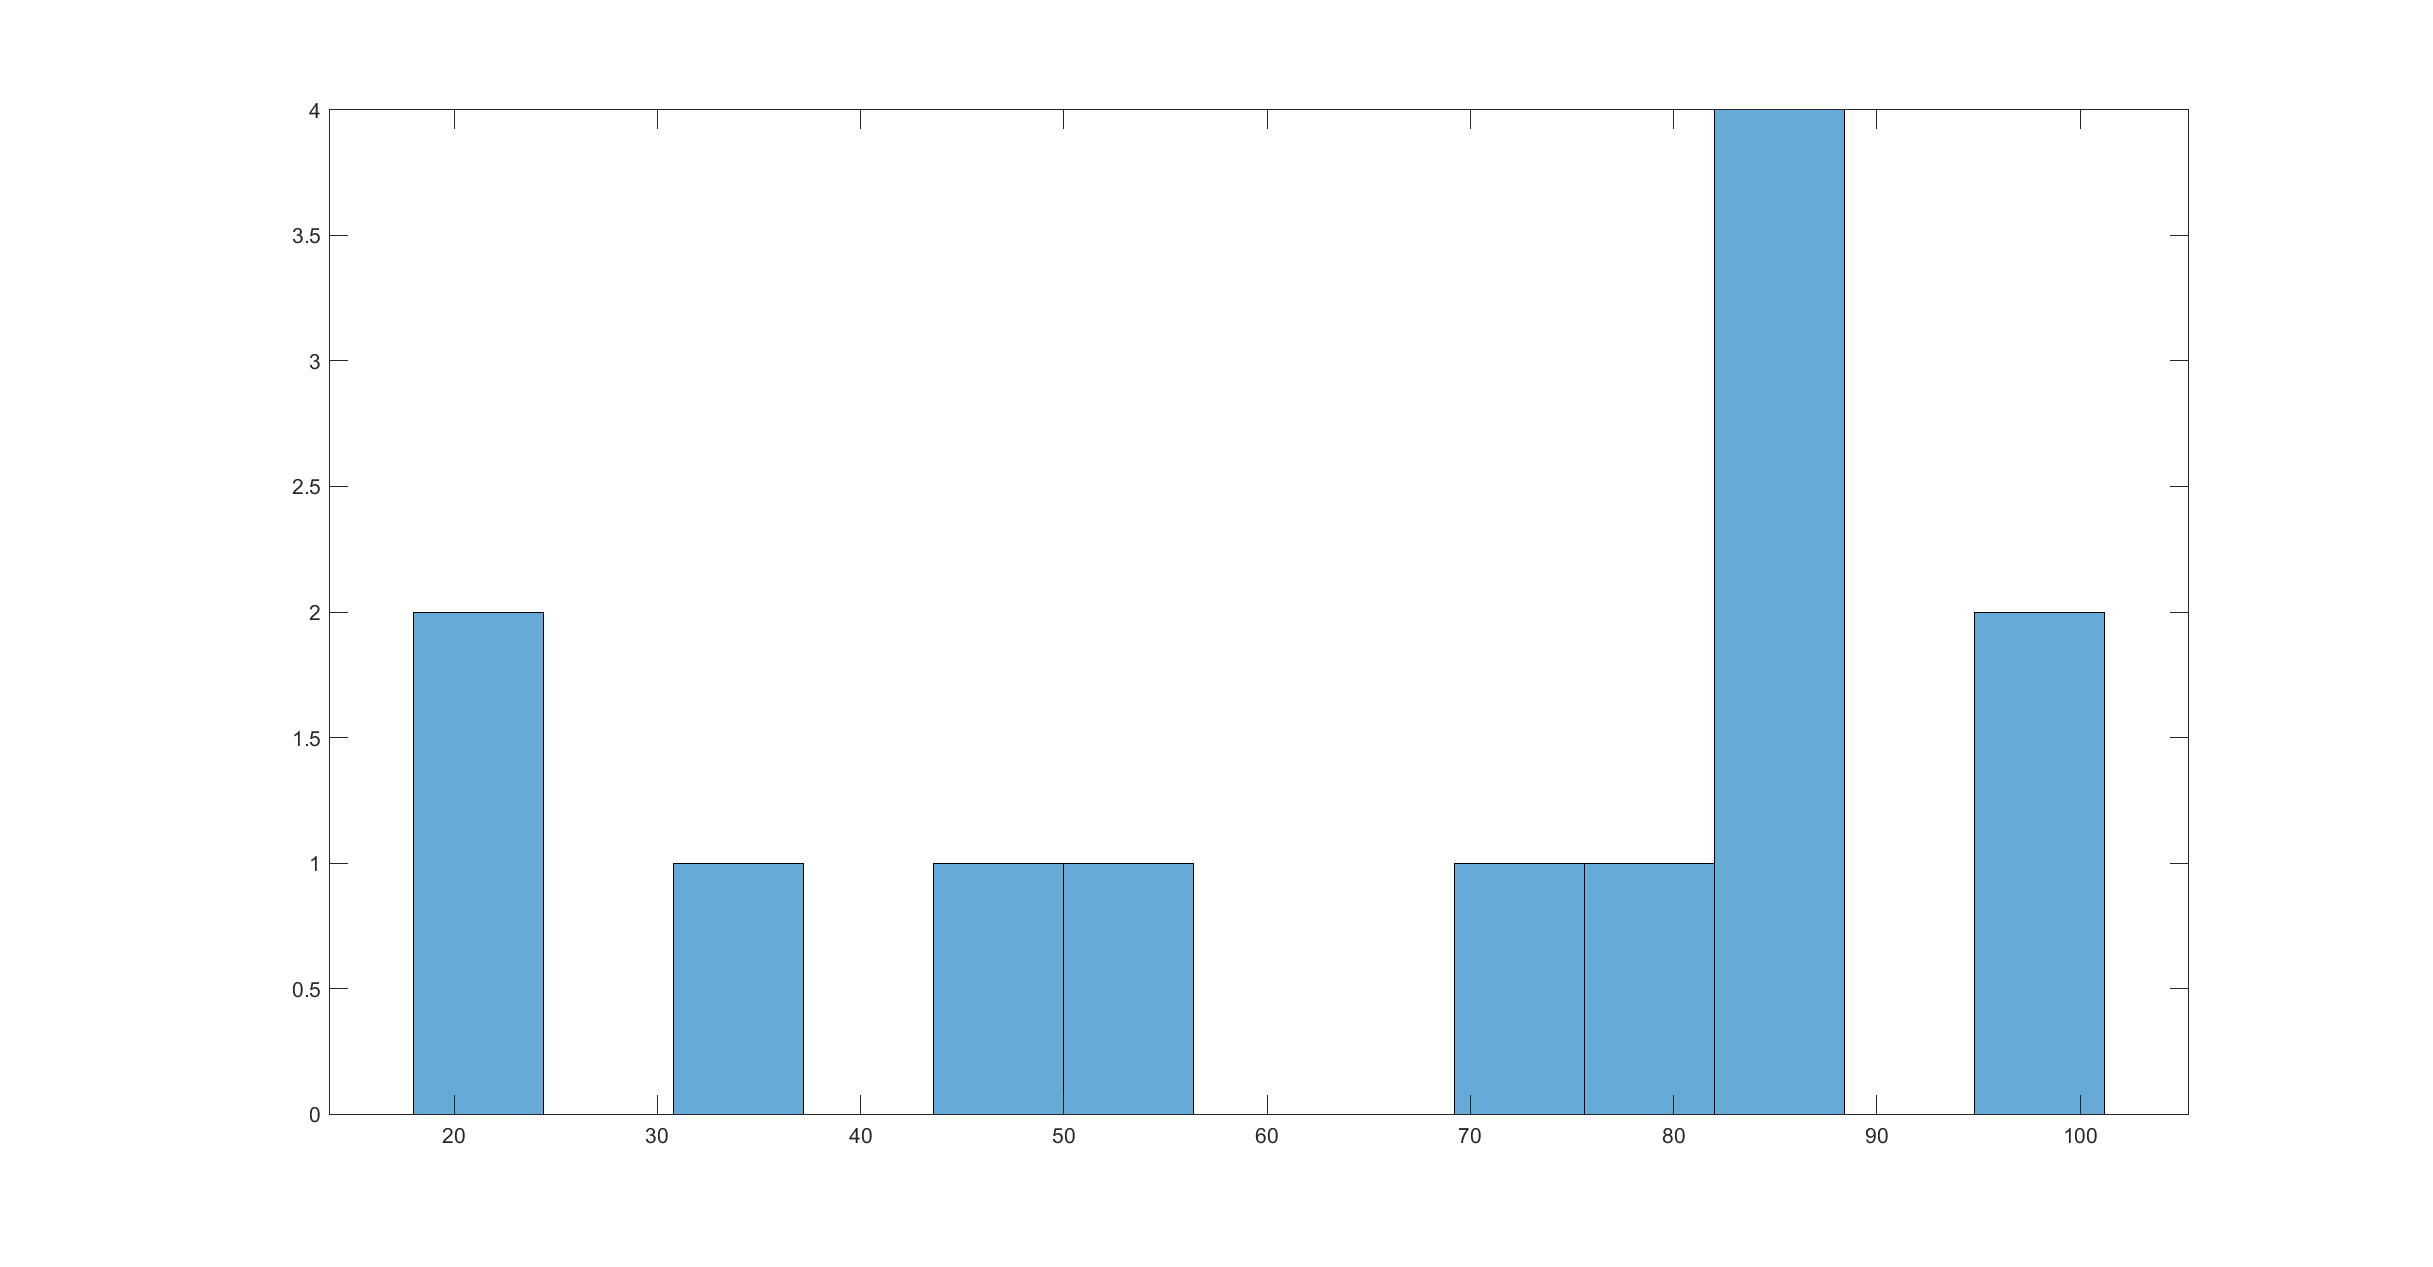
\includegraphics[width=1\linewidth]{untitled.eps}
    \caption{Imagen vectorial}
    \label{fig_vectorial}
\end{center}
\end{figure}

\end{document}
